\documentclass[UTF8,a4paper,12pt]{ctexart}
\usepackage[a4paper,margin=2.2cm]{geometry}
\usepackage{graphicx,float,booktabs,longtable,xcolor,listings,hyperref}
\hypersetup{colorlinks=true,linkcolor=blue,urlcolor=blue}
\setlength{\parindent}{2em}\setlength{\parskip}{0.45em}\sloppy
\newcommand{\shot}[2]{\begin{figure}[H]\centering\includegraphics[width=0.96\textwidth]{截图/#1}\caption{#2}\end{figure}}
\title{计算机网络技术实践实验二报告\\\large PPP串口与静态路由}
\author{学号：已隐去}
\date{2026年10月15日}
\begin{document}\maketitle
\begin{abstract}本实验在Dynamips中使用真实Cisco IOS完成PPP串口协商、DCE时钟配置、静态路由和跨网段互ping，并对PPP链路采集抓包。\end{abstract}
\section{实验要求与目的}
本实验验证路由器基本配置、串口PPP封装、DCE时钟和静态路由。重点不是把以太网链路替换成普通网线，而是从IOS输出确认Serial接口up/up、LCP Open、PPP封装和路由表中的下一跳。
\section{环境与设备}
拓扑包含R1、R2和两台VPCS模拟PC。R1使用Serial1/1作为DCE并配置clock rate 115200，R2使用Serial1/0作为DTE。PC1和PC2分别位于10.2.1.0/24与10.2.2.0/24，串口互联网段为10.2.12.0/30。Dynamips虚拟串口不需要实体DCE/DTE线缆。
\begin{figure}[H]\centering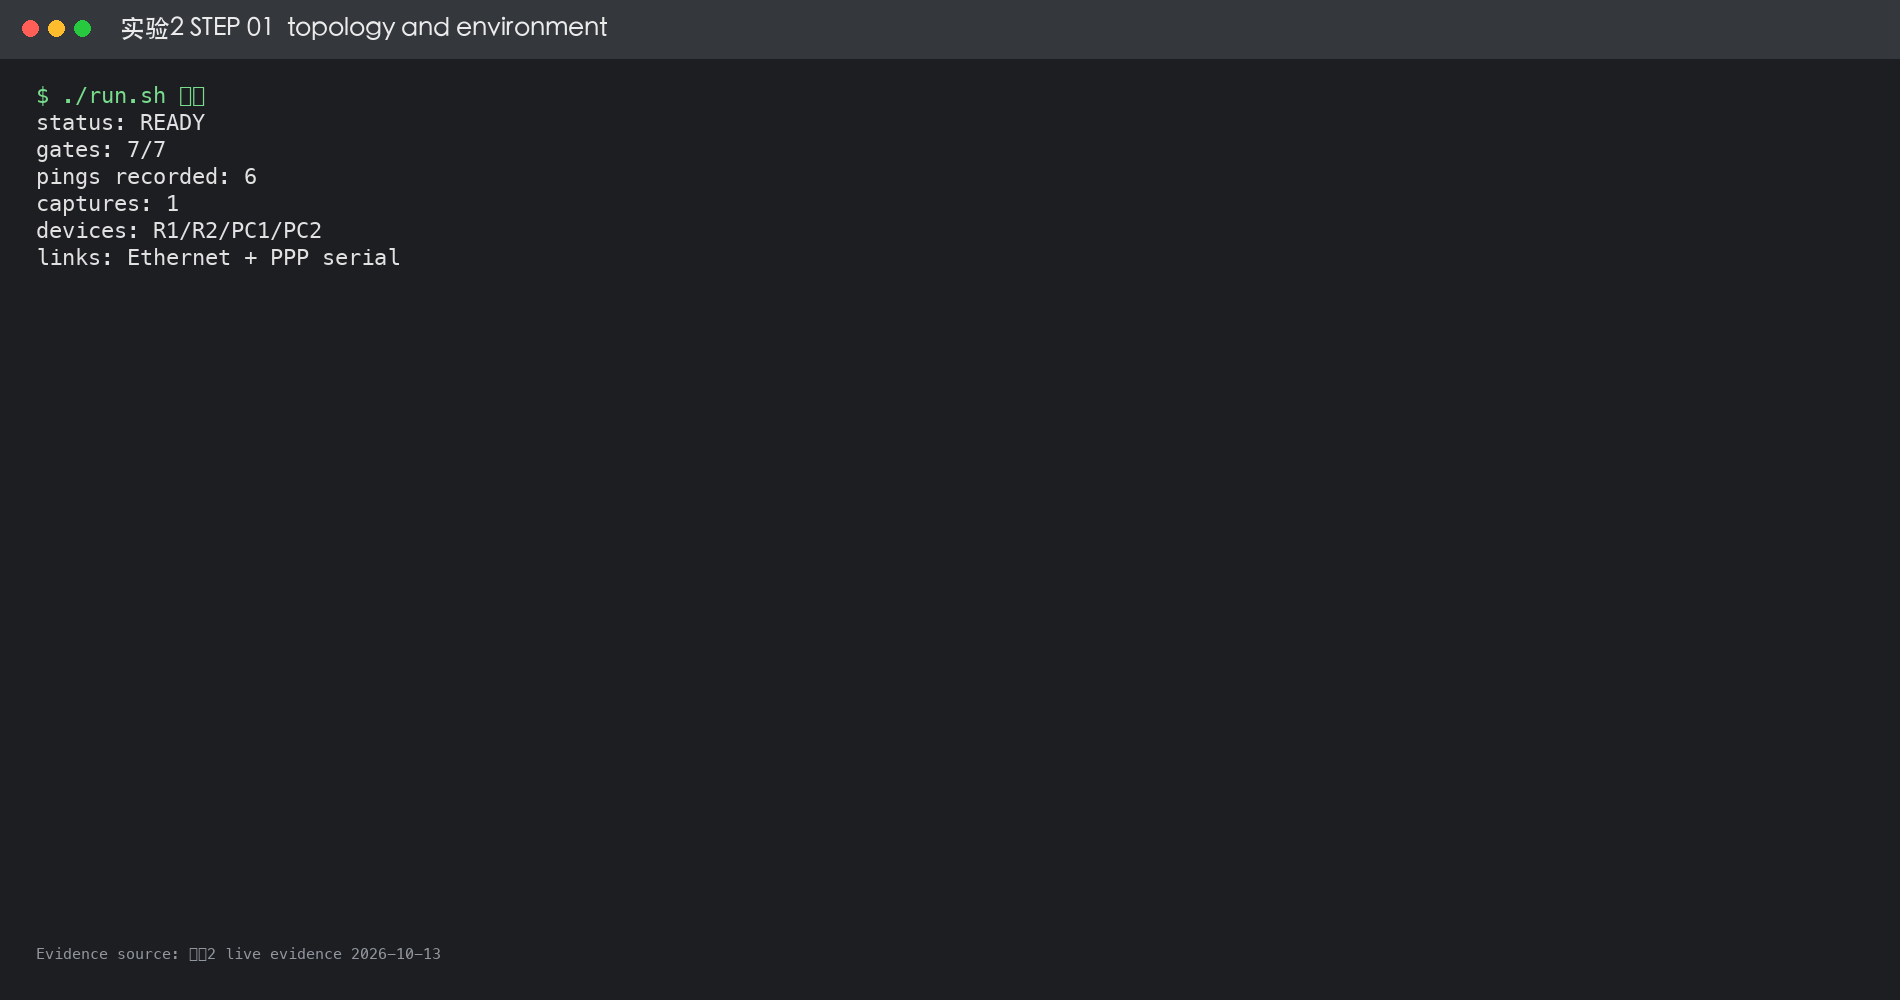
\includegraphics[width=0.96\textwidth]{截图/01-环境与拓扑预检.png}\caption{设备和链路验收摘要。}\end{figure}
\section{配置思路}
先启动四个IOS实例，再配置两端以太网接口和串口地址；DCE侧设置时钟并启用PPP；随后在两台路由器上添加对端LAN的静态路由，在PC上设置默认网关。配置顺序先接口、后路由、再连通性，可以避免把路由缺失误判成PPP故障。
\begin{figure}[H]\centering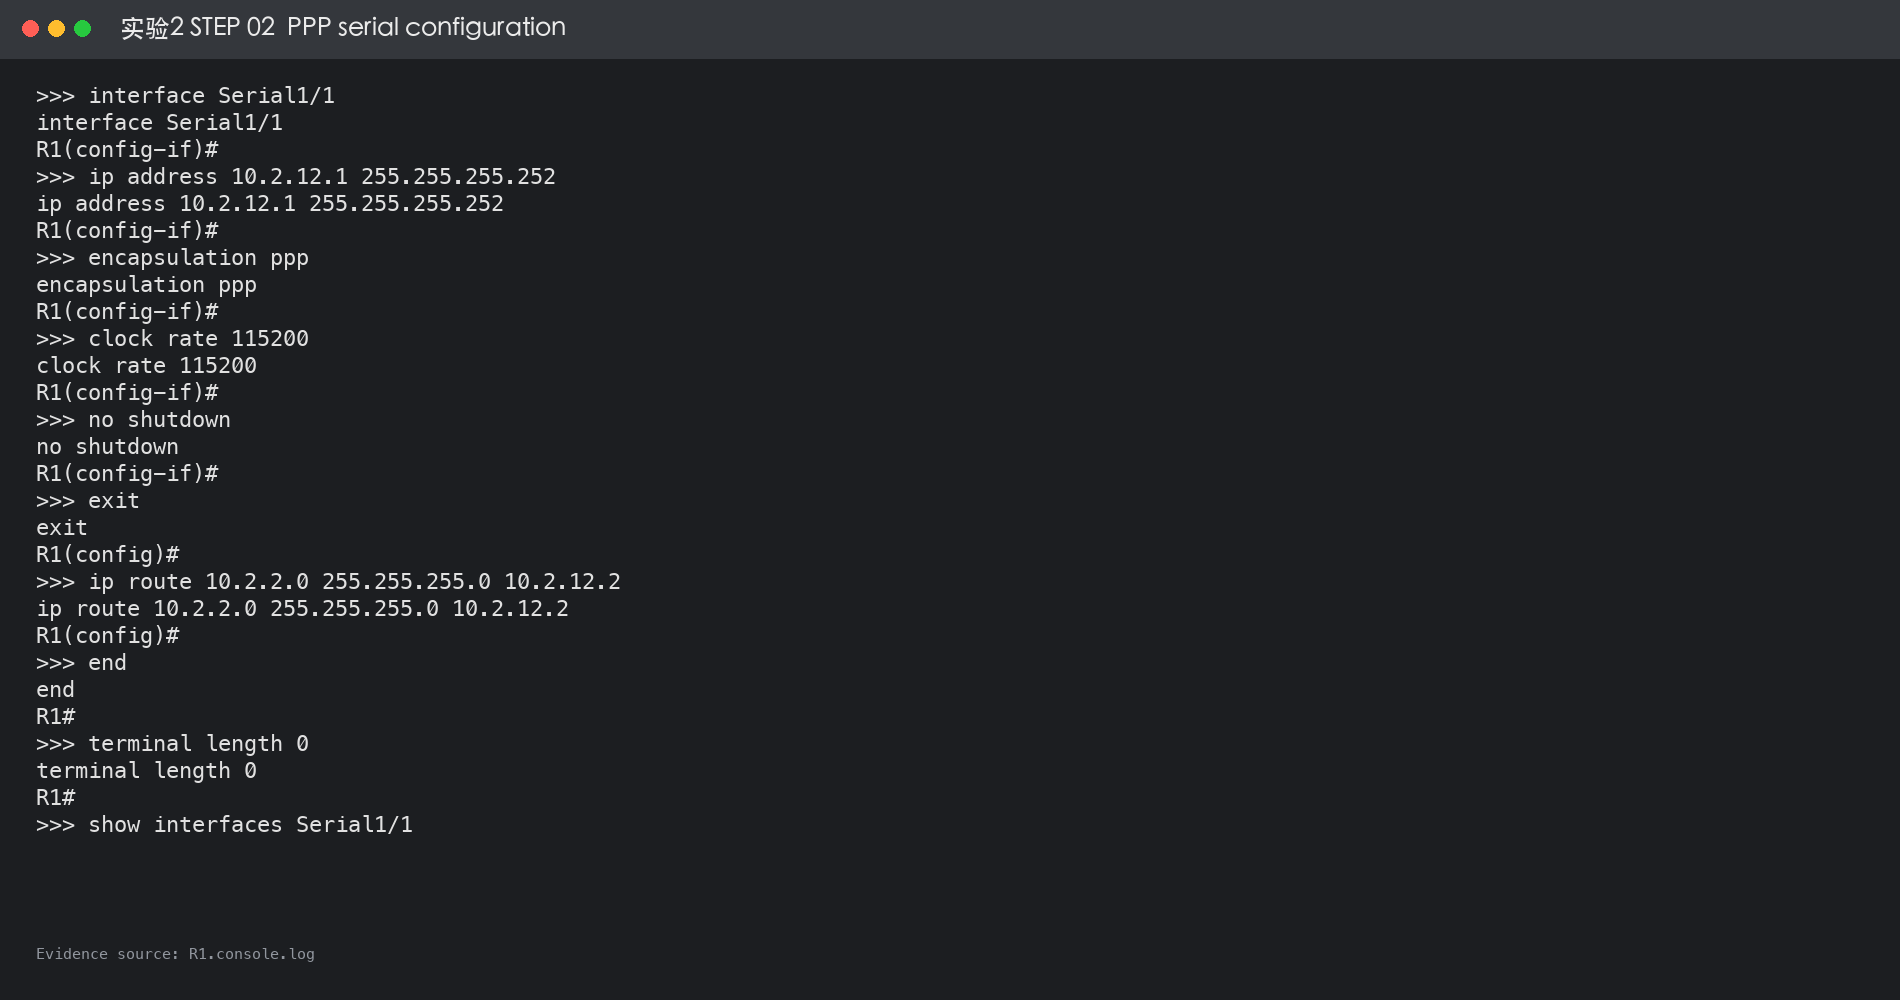
\includegraphics[width=0.96\textwidth]{截图/02-PPP配置.png}\caption{R1串口PPP和DCE时钟配置。}\end{figure}
\section{验证过程}
执行show interfaces Serial1/1、show interfaces Serial1/0确认line protocol up、Encapsulation PPP和LCP Open；执行show ip route确认静态路由；PC两方向各连续三轮ping，先预热ARP后统计正式结果，并采集PPP链路抓包。
\begin{figure}[H]\centering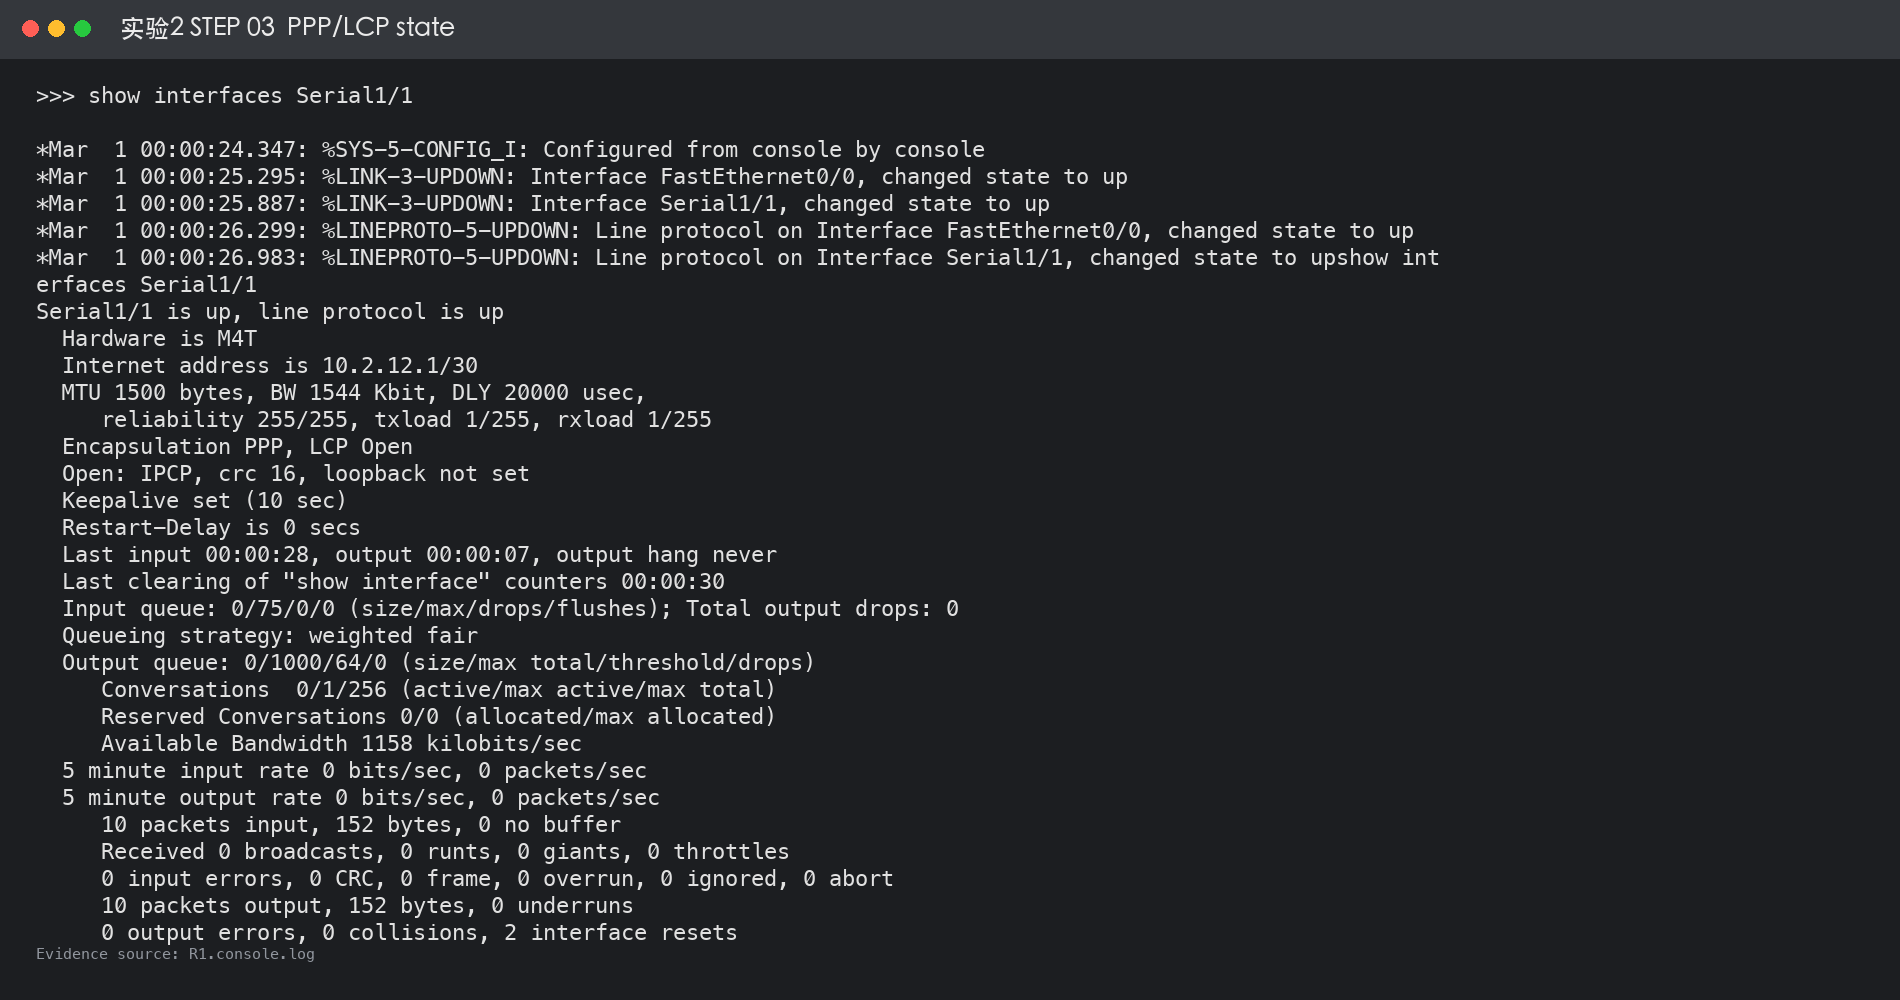
\includegraphics[width=0.96\textwidth]{截图/03-PPP状态.png}\caption{串口PPP状态和LCP协商。}\end{figure}
\section{结果分析}
历史通过证据中四台设备和三条链路门禁通过，PPP/LCP、clock rate、静态路由和PPP抓包门禁均通过；PC1到10.2.2.2、PC2到10.2.1.2均达到100%（5/5）。抓包用于证明链路上确实出现PPP封装后的ICMP，而不是只检查配置文本。
\begin{figure}[H]\centering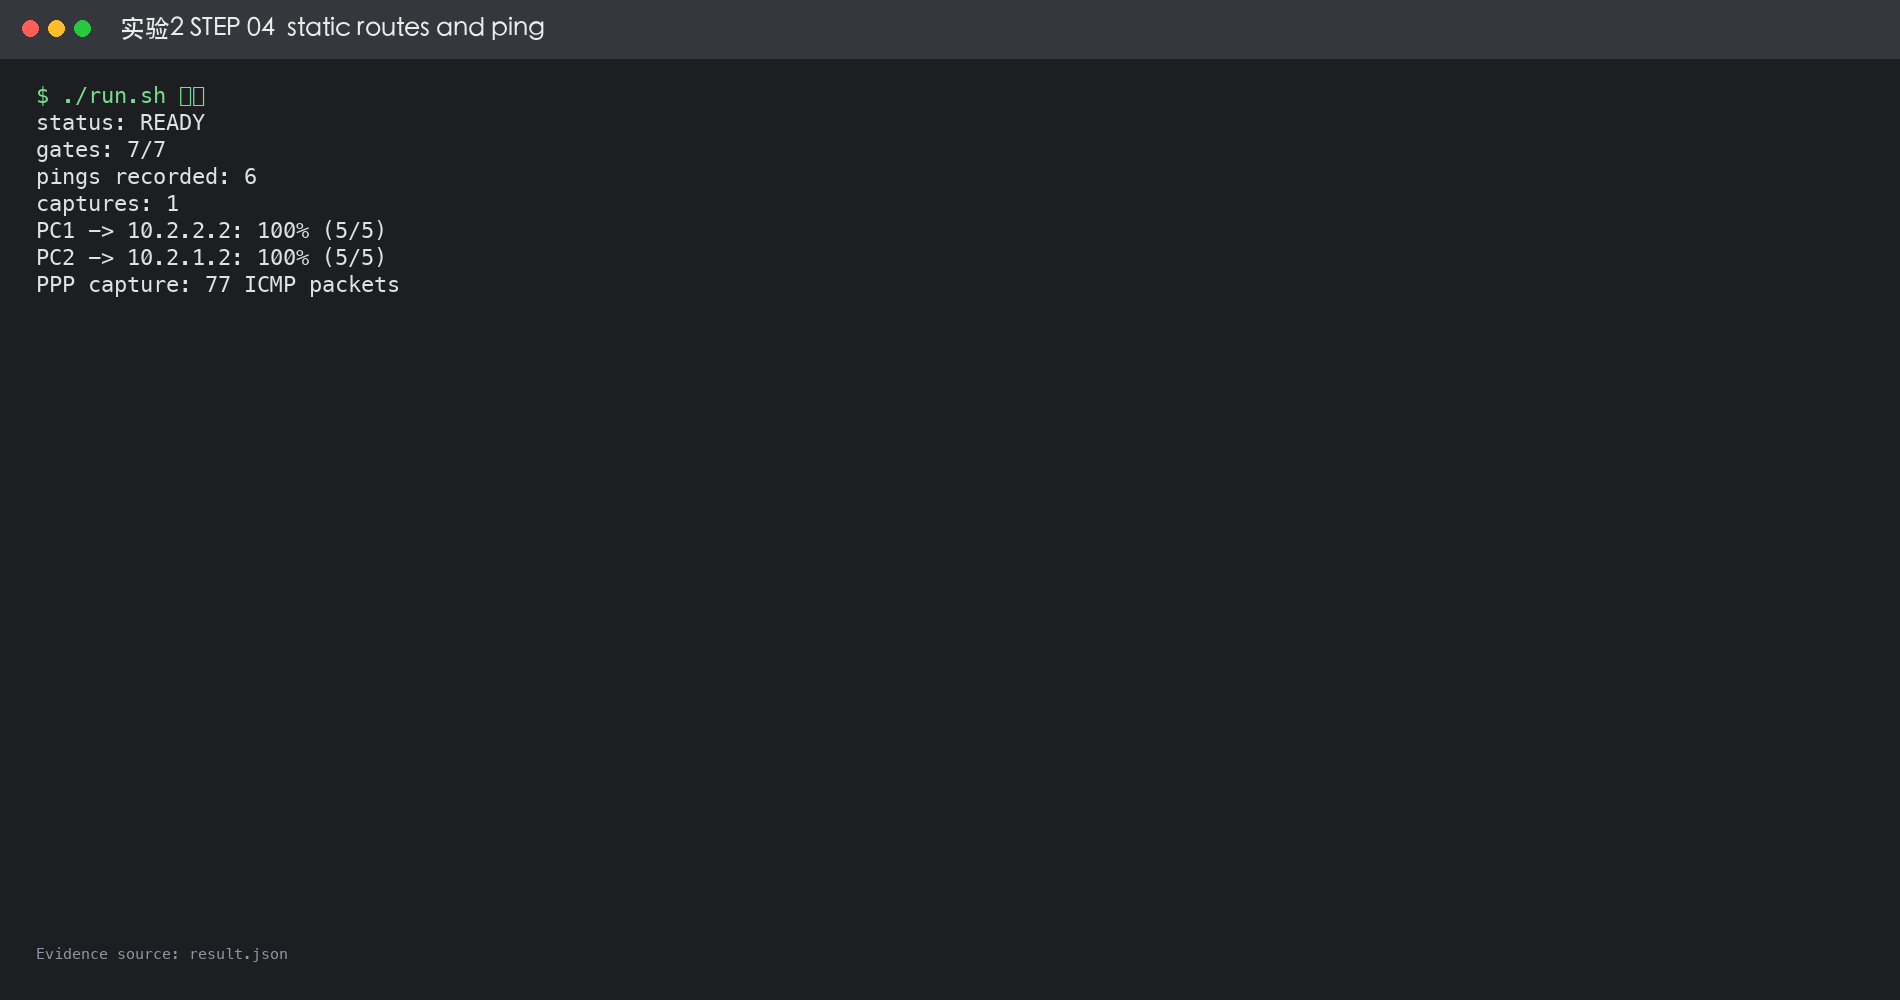
\includegraphics[width=0.96\textwidth]{截图/04-静态路由互ping.png}\caption{静态路由和双向互ping结果。}\end{figure}
\section{失败与修正记录}
首次运行因命令回显空格规则导致超时，随后修正匹配规则并从空状态重跑取得READY。报告采用通过运行的result.json，同时保留首次失败证据，便于复盘。
\section{截图与证据边界}
本报告的终端图由本项目实际Dynamips/Cisco IOS运行日志和验收JSON生成，原始证据目录保留在本实验的\texttt{evidence/}中。截图展示命令与回显，不把上游报告结果当作本实验结果。当前状态为\textbf{READY}。
\section{结论}
本实验已取得完整通过证据，结论可由结果JSON、控制台日志和抓包文件复核。

\end{document}
